\section{روند کد‌ها}
\begin{frame}[fragile]{کد کامپایل می‌شود}
\begin{itemize}\itemr
\item[-]
فرض کنید شما متد
\lr{\texttt{list.sort()}}
را در خطی از کد‌های خودتان صدا زده‌اید:

\begin{latin}
\begin{lstlisting}[language=python]
data = list(generate_data())
data.sort()
\end{lstlisting}
\end{latin}

\item[-]
چنین بایت‌کدی برای کد شما زمان کامپایل تولید شده است:

\begin{latin}
\begin{lstlisting}
  1           0 LOAD_NAME                0 (list)
              2 LOAD_NAME                1 (generate_data)
              4 CALL_FUNCTION            0
              6 CALL_FUNCTION            1
              8 STORE_NAME               2 (data)
             10 LOAD_NAME                2 (data)
             12 LOAD_METHOD              3 (sort)
             14 CALL_METHOD              0
             16 POP_TOP
             18 LOAD_CONST               0 (None)
             20 RETURN_VALUE
\end{lstlisting}
\end{latin}
\end{itemize}
\end{frame}

\begin{frame}[fragile]{متد \lr{load} می‌شود}
\begin{flushright}
اول نام متد گرفته می‌شود، و سپس توسط 
\lr{\texttt{\_PyObject\_GetMethod}}
پیدا می‌شود. اگر نبود \lr{error} اتفاق میوفتد.
\end{flushright}
\begin{figure}[H]
\begin{center}
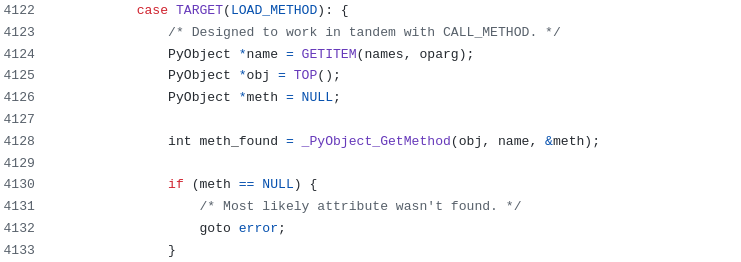
\includegraphics[width=0.8\textwidth, height=0.5\textheight]{docs/images/load-1}
\end{center}
\end{figure}
\end{frame}

\begin{frame}[fragile]{متد \lr{load} می‌شود}
\begin{flushright}
چون 
\lr{CPython}
یک ماشین مجازی \lr{stack based} است، آبجکت 
\lr{\texttt{self}}
و خود متد، روی استک
\lr{push}
می‌شوند.
\end{flushright}
\begin{figure}[H]
\begin{center}
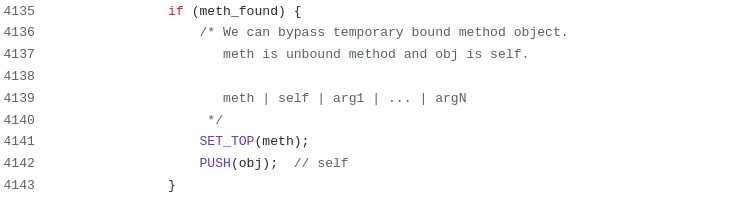
\includegraphics[width=0.8\textwidth, height=0.4\textheight]{docs/images/load-2}
\end{center}
\end{figure}
\end{frame}

\begin{frame}{متد صدا زده می‌شود}
\begin{figure}[H]
\begin{center}
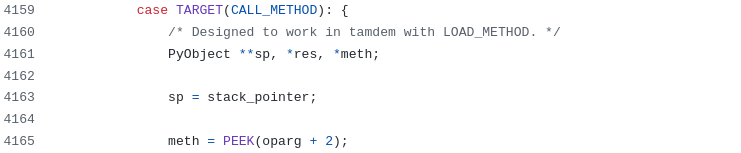
\includegraphics[width=0.8\textwidth, height=0.3\textheight]{docs/images/call-1}
\end{center}
\end{figure}
\end{frame}

\begin{frame}{متد صدا زده می‌شود}
\begin{flushright}
حالا متغیر‌های لازم به 
\lr{\texttt{call\_function}}
پاس داده می‌شوند تا کار صدا زدن متد را انجام بدهد.
\end{flushright}
\begin{figure}[H]
\begin{center}
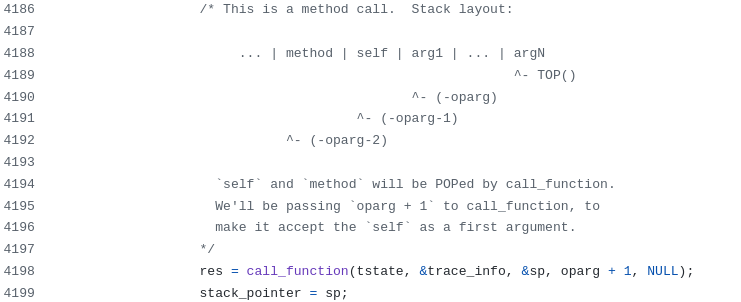
\includegraphics[width=0.8\textwidth, height=0.65\textheight]{docs/images/call-2}
\end{center}
\end{figure}
\end{frame}

\begin{frame}{متد صدا زده می‌شود}
\begin{flushright}
تابع 
\lr{\texttt{call\_function}}
این تابع را صدا می‌زند.
\end{flushright}
\begin{figure}[H]
\begin{center}
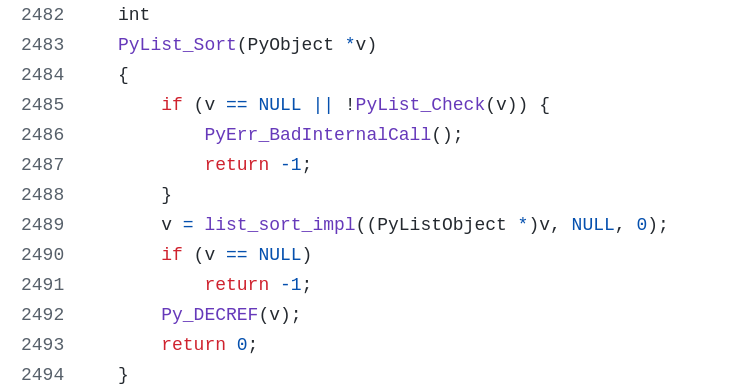
\includegraphics[width=0.8\textwidth, height=0.6\textheight]{docs/images/PyList_Sort}
\end{center}
\end{figure}
\end{frame}

